
\begin{center}
	\LARGE
	Uden hjælpemidler
\end{center}
\begin{opgavetekst}{Opgave 1}
	\begin{center}
		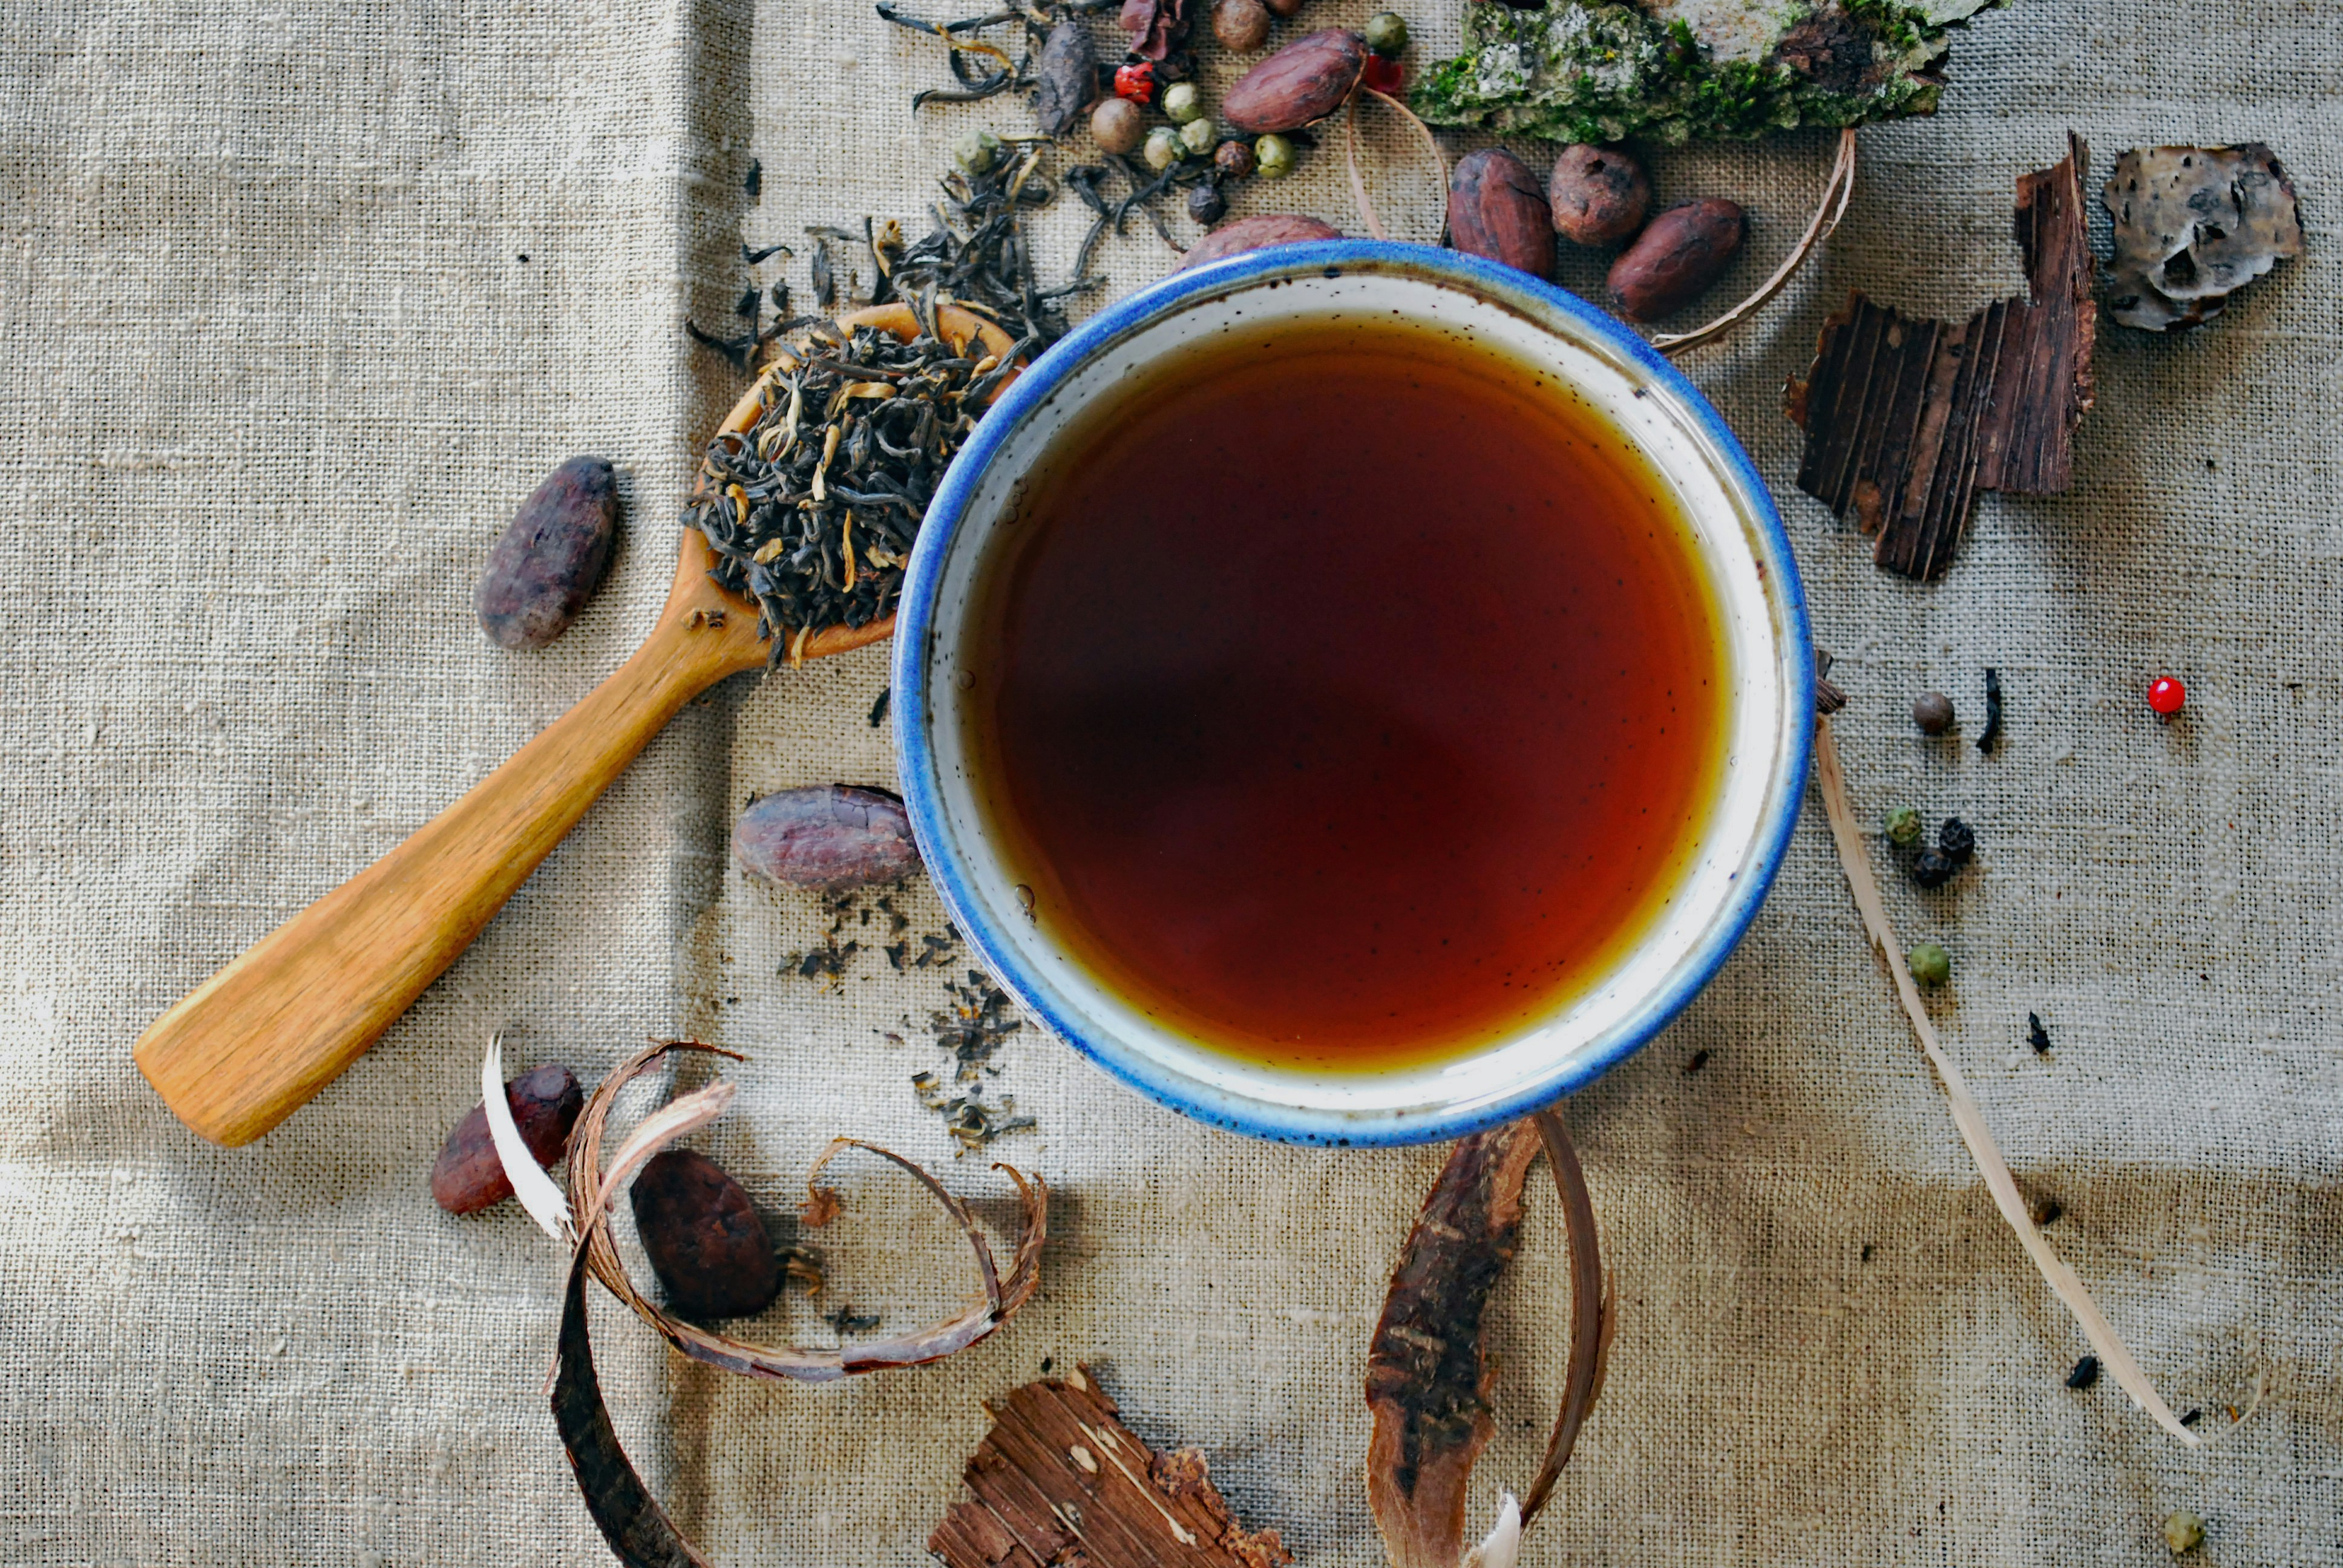
\includegraphics[width=0.6\textwidth]{Billeder/te}
	\end{center}
	Du tager en kop te med udenfor. Teens temperatur kan beskrives ved funktionen $f$ givet ved
	\begin{align*}
		f(t) = 85.6\cdot 0.931^t,
	\end{align*}
	hvor $t$ betegner antallet af forløbne minutter siden du bryggede teen, og $f$ betegner temperaturen af teen i
	 C$^\circ$.
\end{opgavetekst}
\begin{delopgave}{1}
	Forklar, hvad tallene $85.6$ og $0.931$ siger om temperaturen af teen.
\end{delopgave}

\begin{opgavetekst}{Opgave 2}
	En eksponentialfunktion $g$ er givet ved
	\begin{align*}
		g(x) = 2\cdot 5^x
	\end{align*}
\end{opgavetekst}
\begin{delopgave}{1}
	Løs ligningen $g(x) = 250$.
\end{delopgave}

\begin{opgavetekst}{Opgave 3}
	En potensfunktion $h$ opfylder, at $h(2) = 4$, og $h(8) = 256$.
\end{opgavetekst}
\begin{delopgave}{1}
	Bestem en forskrift for $h$. (Vink: Overvej, om andre logaritmer er smartere at bruge end $\log_{10}$).
\end{delopgave}
\begin{delopgave}{2}
	Bestem tallet $h(5)$.
\end{delopgave}

\begin{opgavetekst}{Opgave 4}
	\begin{center}
		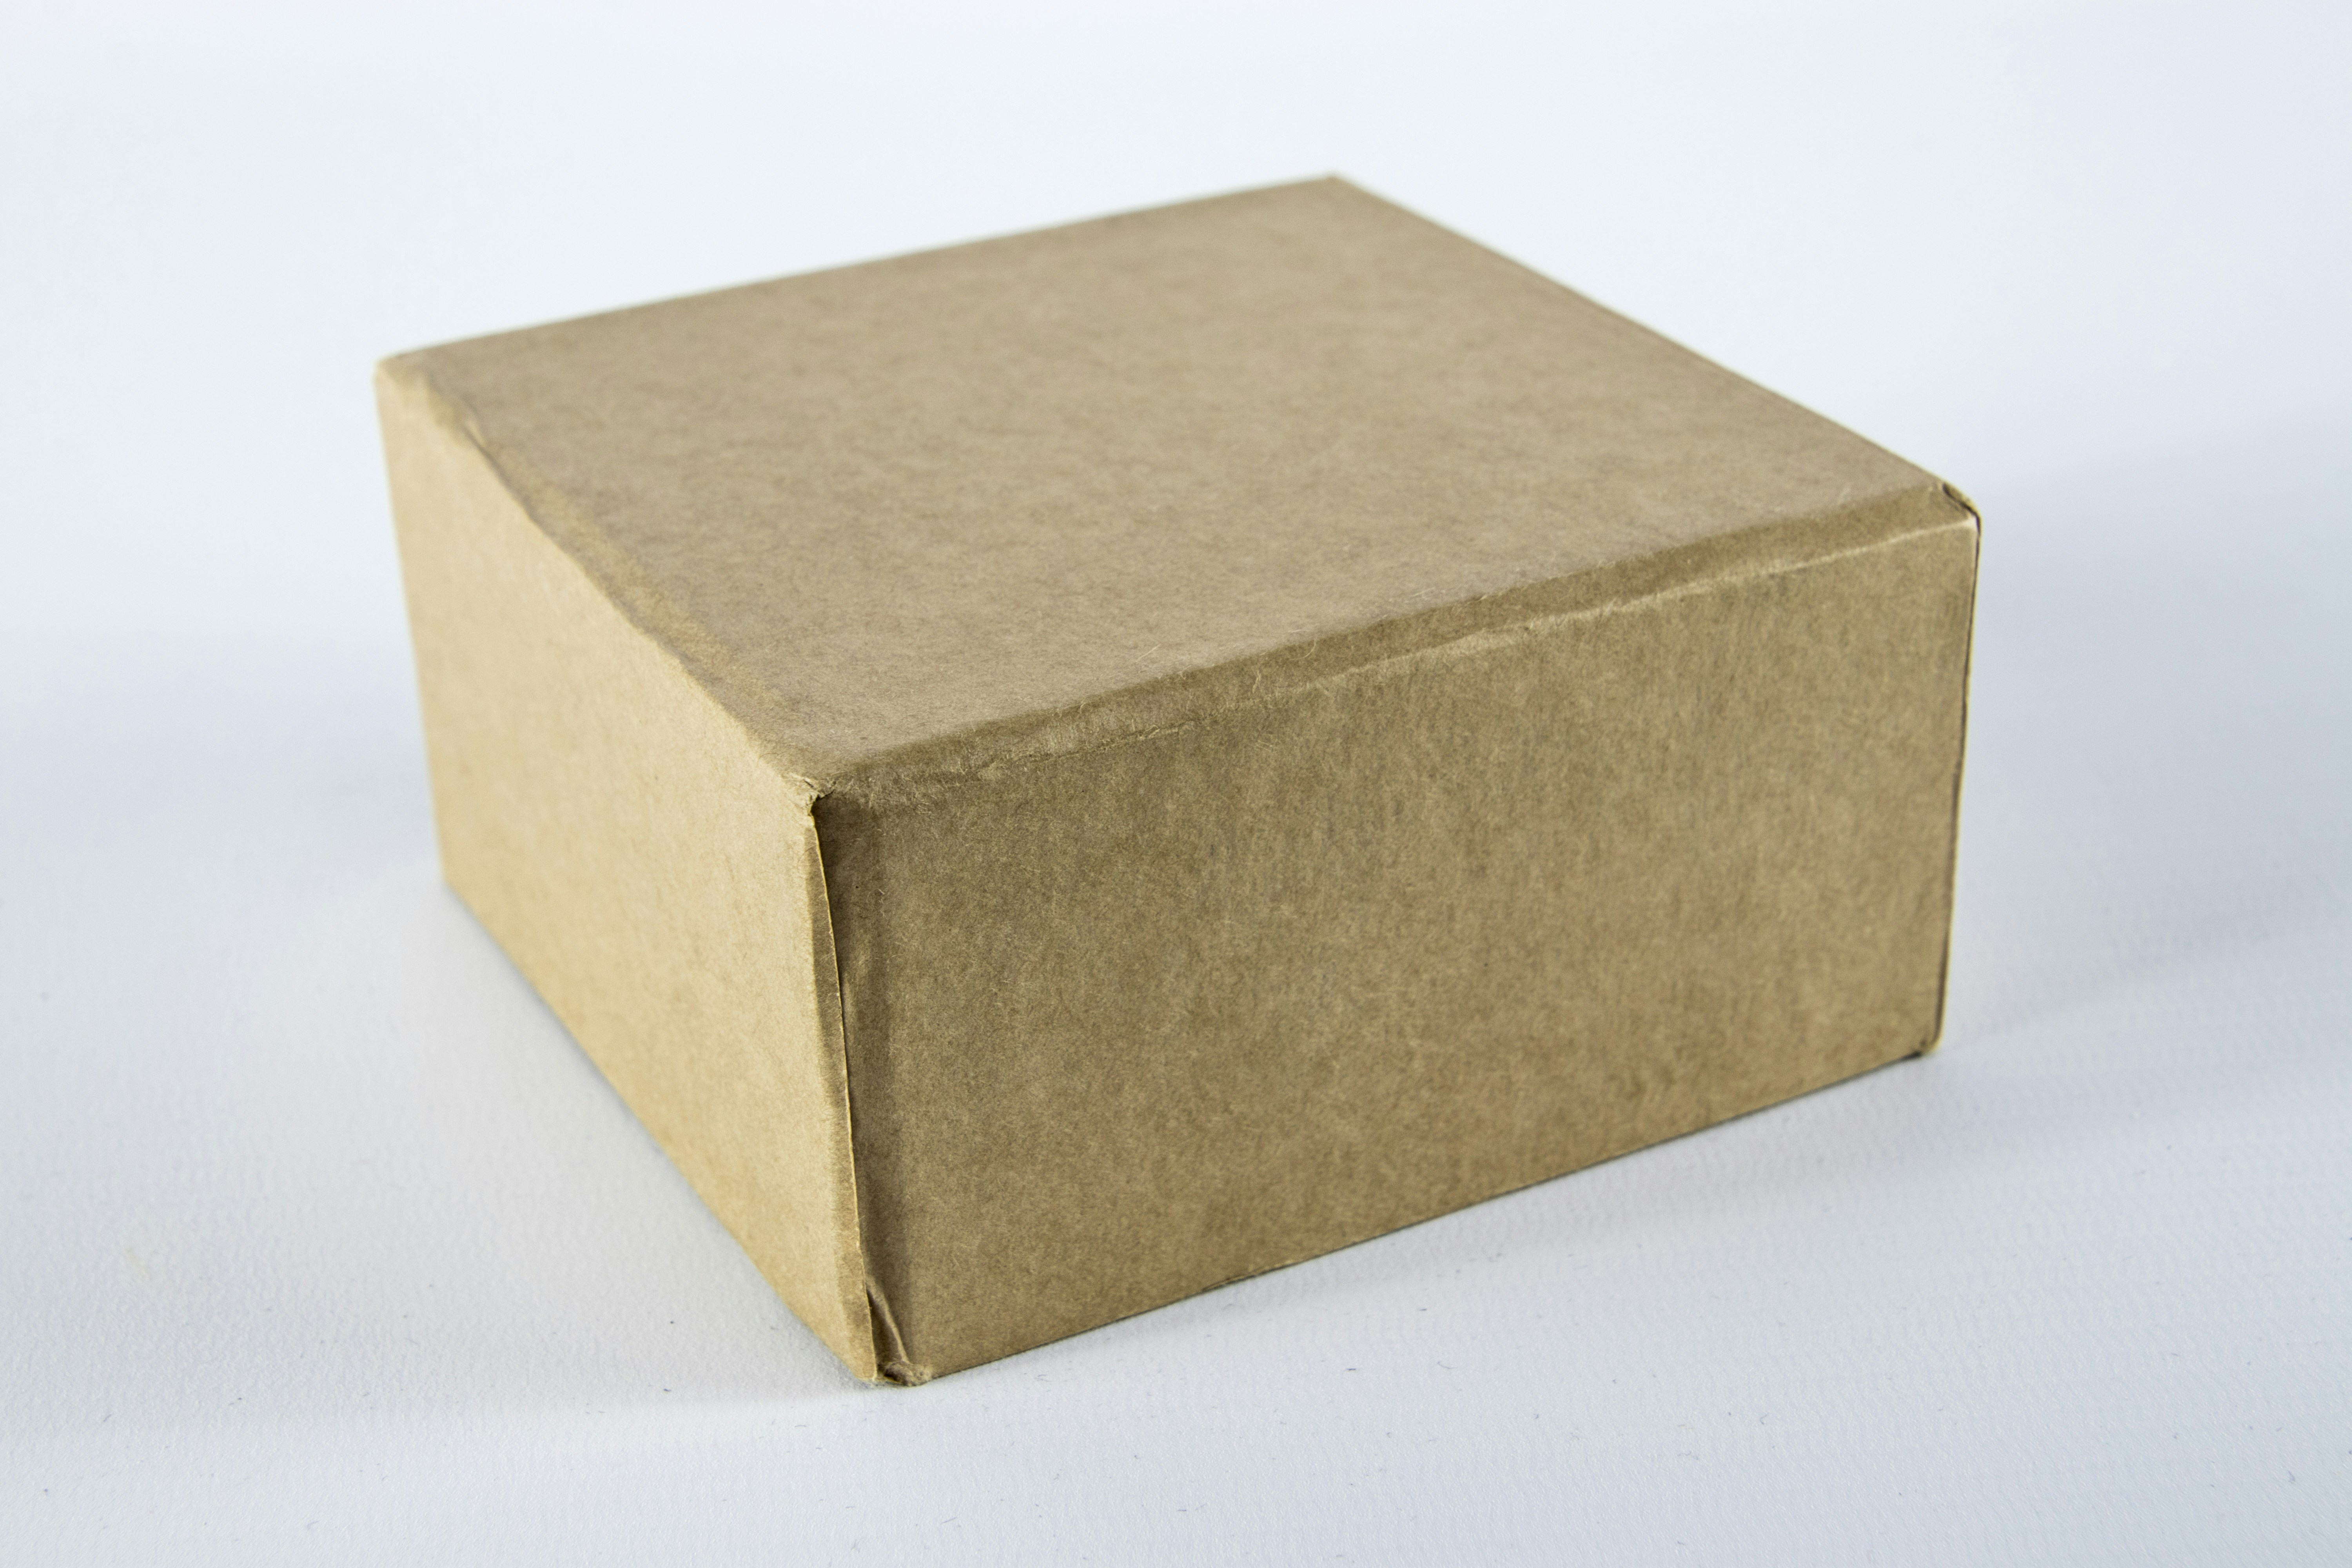
\includegraphics[width = 0.55\textwidth]{Billeder/kasse}
	\end{center}
	En kasse til pakketransport opfylder at have en kvadratisk bund. Den er desuden dobbelt så bred som den er høj, og
	højden af kassen betegnes med $x$.
\end{opgavetekst}
\begin{delopgave}{1}
	Opskriv en funktion $R$, der beskriver rumfanget af kassen som funktion af $x$.
\end{delopgave}
\begin{delopgave}{2}
	Hvis alle dimensioner af kassen firedobles, hvor mange gange større bliver rumfanget af kassen så?
\end{delopgave}
\begin{opgavetekst}{Opgave 5}
	Grafen for en eksponentialfunktion $g$ kan ses på Figur \ref{fig:exp}.
	\begin{figure}[H]
		\centering
		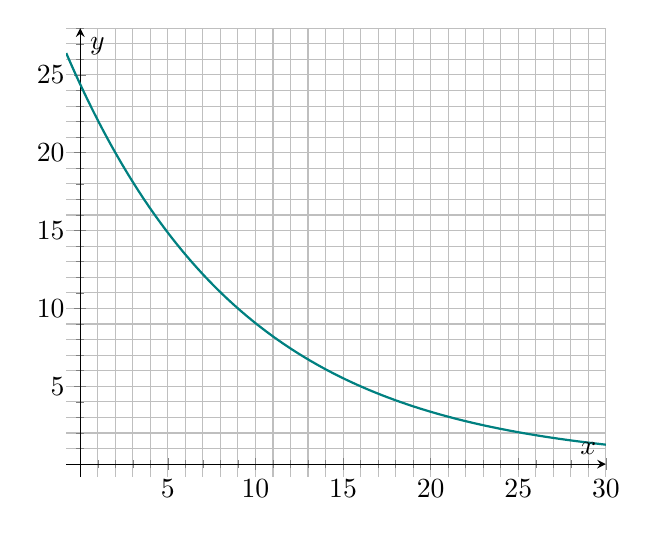
\begin{tikzpicture}
			\begin{axis}[
				axis lines = center,
				xmin = -0.8, xmax = 30,
				ymin = -0.8,ymax = 28,
				grid = both,
				minor tick num = 4,
				xlabel = $x$, ylabel = $y$
			]
				\addplot[thick, samples = 1000, color = teal, domain = -0.8:40] {24.390*0.90572^x};
			\end{axis}
		\end{tikzpicture}
		\caption{Grafen for eksponentialfunktionen $g$.}
		\label{fig:exp}
	\end{figure}
	\phantom{h}
\end{opgavetekst}
\begin{delopgave}{1}
	Aflæs halveringskonstanten for $g$. 
\end{delopgave}
\newpage

\begin{center}
	\LARGE
	Med hjælpemidler
\end{center}

\begin{opgavetekst}{Opgave 6}
	\begin{center}
		
\includegraphics[width=0.6\textwidth]{Billeder/boble}
	\end{center}
	Du ønsker dig en bil og har besluttet dig for at spare op til den. Du opsparer månedligt 2000 kr og skal efter 5 år
	have opsparet $135\TS 000$kr. 
\end{opgavetekst}
\begin{delopgave}{1}
	Hvad skal din månedlige rente være, hvis du efter 5 år skal have opsparet dette beløb? 
	(Vink: Brug reelSolve)
\end{delopgave}
\begin{delopgave}{2}
	Hvad tilsvarer denne rente i årlig rente?
\end{delopgave}

\newpage
\begin{opgavetekst}{Opgave 7}
	\begin{center}
		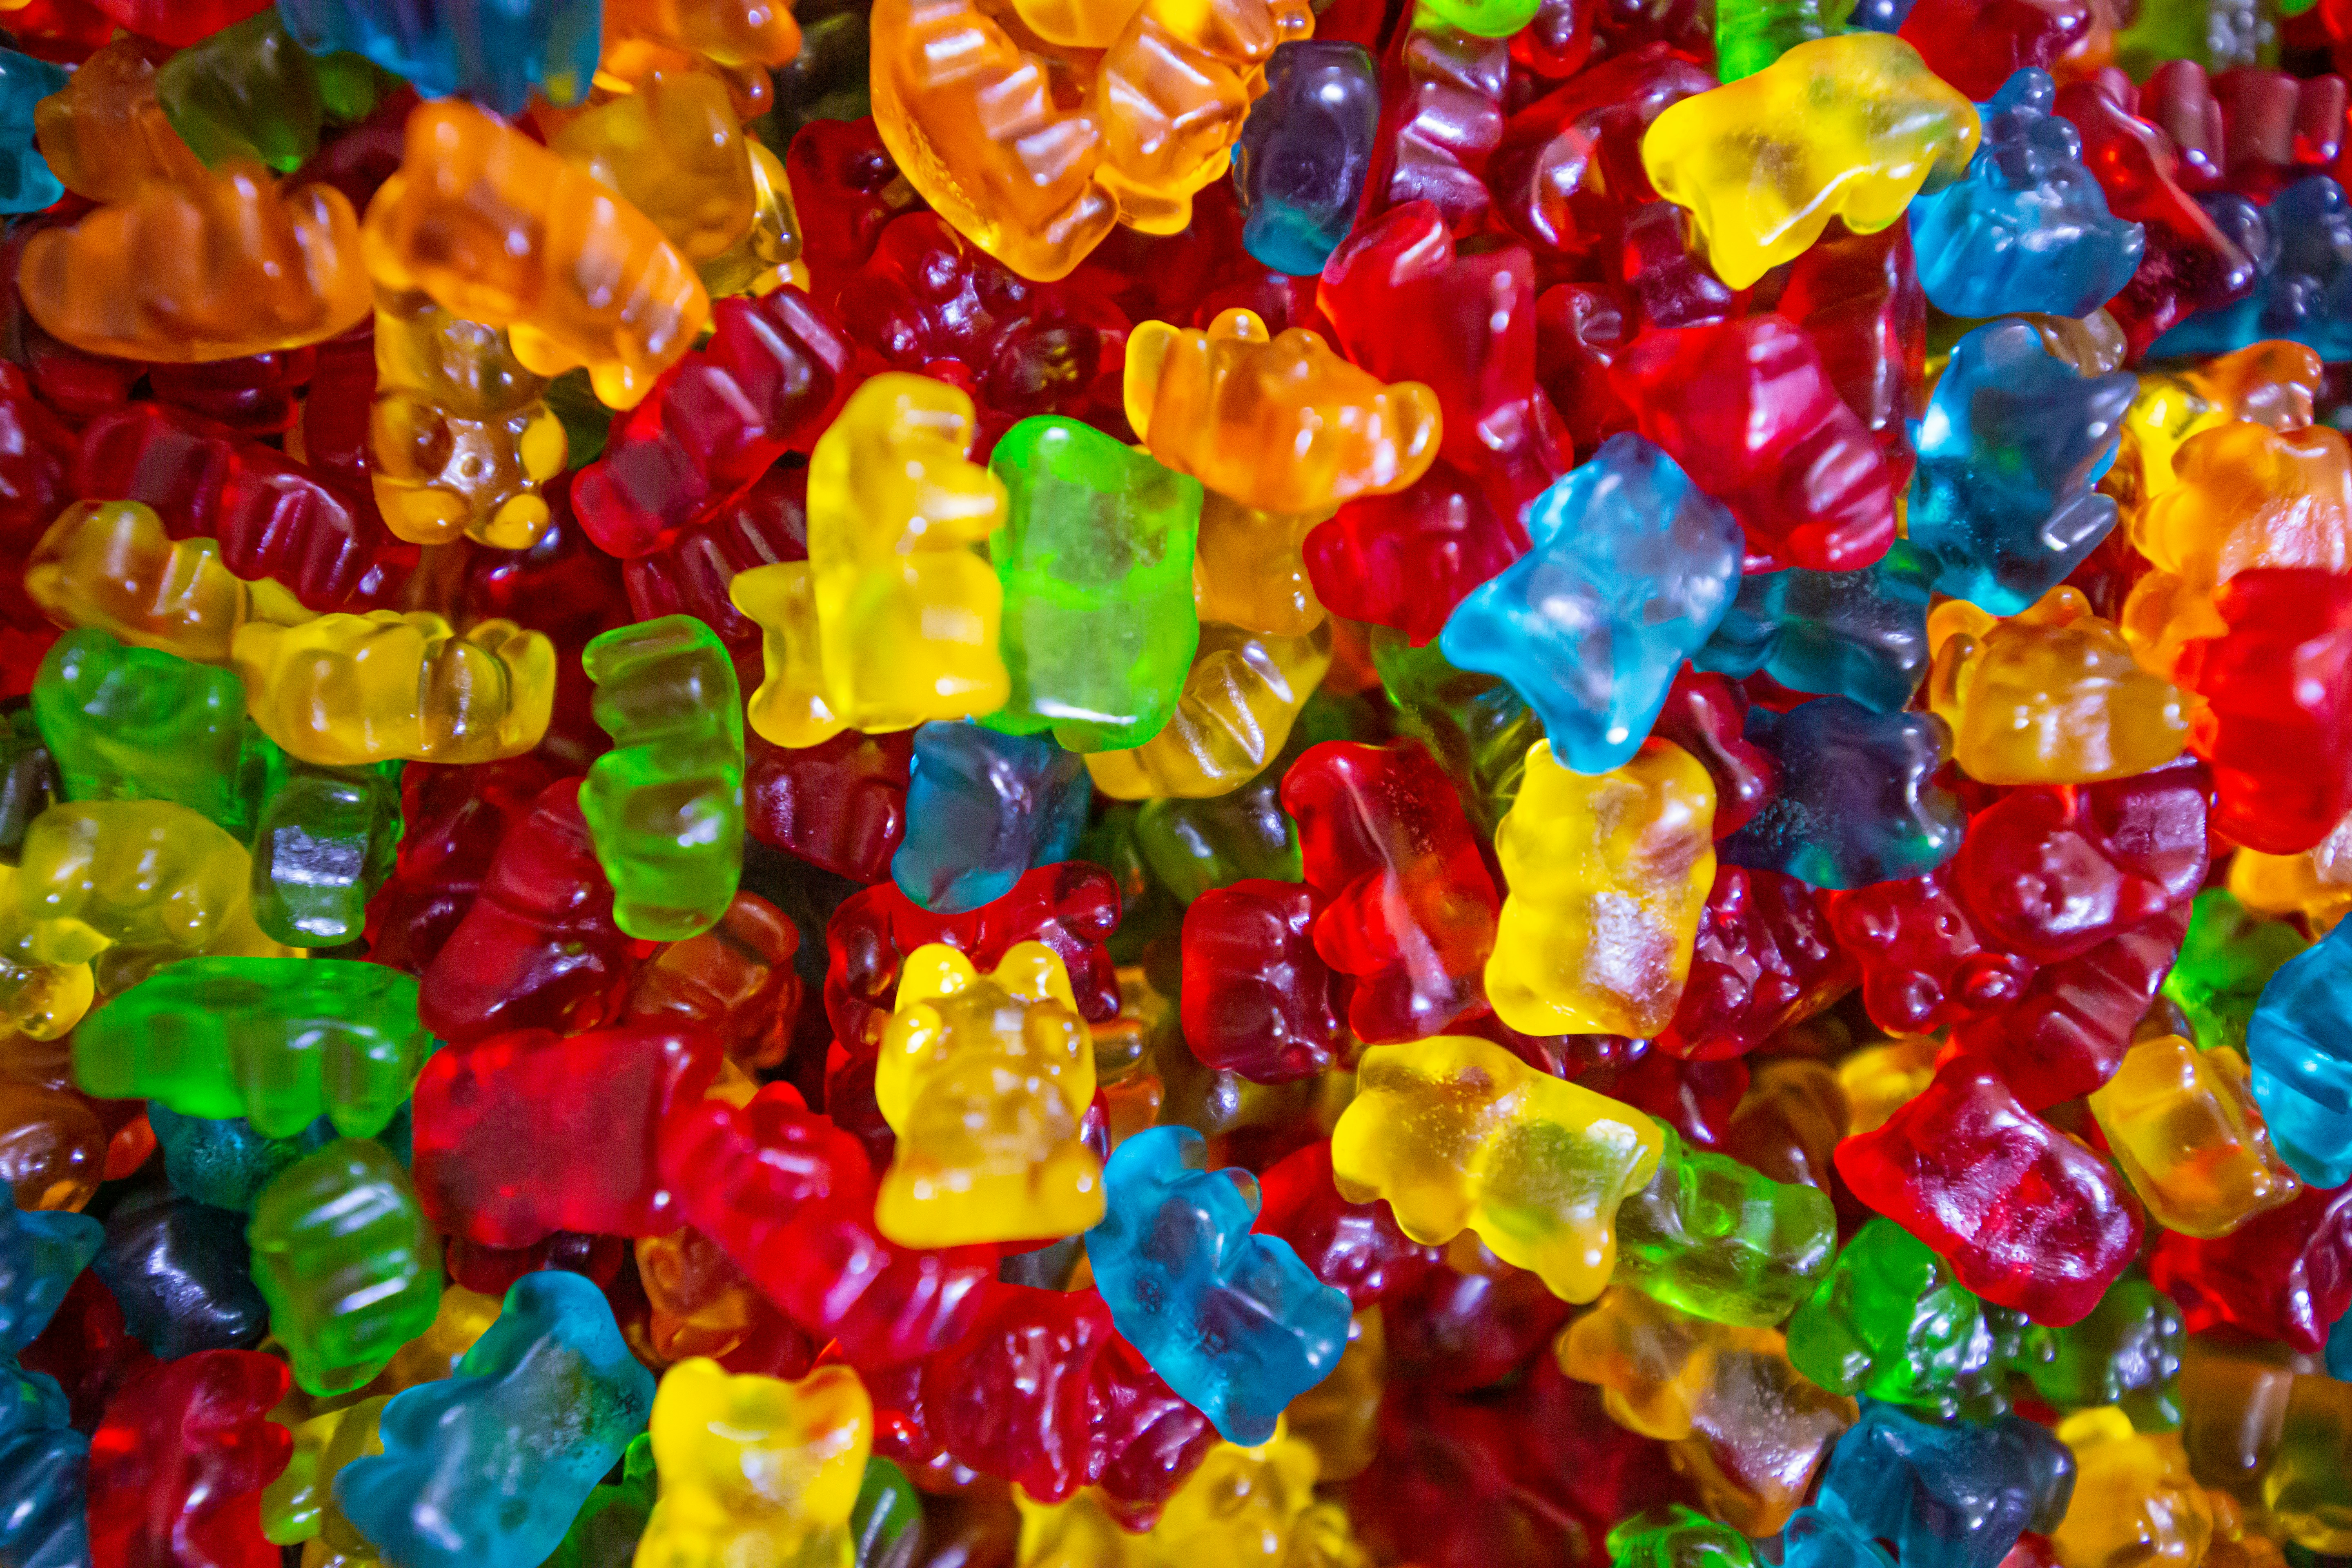
\includegraphics[width = 0.55\textwidth]{Billeder/slik}
	\end{center}
	En gruppe gymnasieelever har målt diameteren af forskellige stykker nogenlunde runde stykker slik og har derefter vejet dem. De forventer, at sammenhængen mellem slikkets 
	diameter $x$ i mm og vægten af slikket $g$ i gram kan beskrives ved en sammenhæng af typen
	\begin{align*}
		g(x) = b \cdot x^a.
	\end{align*}	 
	Resultatet af deres dataindsamling kan findes \href{https://github.com/ChristianJLex/TeachingNotes/raw/master/2023-2024/Data%20og%20lign/Slikvaegt.xlsx}{\color{blue!60} her.}
\end{opgavetekst}
\begin{delopgave}{1}
	Brug datasættet til at bestemme tallene $a$ og $b$.
\end{delopgave}
\begin{delopgave}{2}
	Bestem vægten af et stykke slik med en diameter på 20mm.
\end{delopgave}
\begin{meretekst}
	Bent påstår, at han kan spise et stykke slik på 100g i én mundfuld. De andre udviser en vis skepsis og beder derfor Bent om at åbne munden, så de kan 
	måle, hvor stor afstanden fra hans tænder er. De måler afstanden til at være 30mm. 
\end{meretekst}
\begin{delopgave}{3}
	Afgør, om Bent rent faktisk kan gabe over et stykke slik på 100g. 
\end{delopgave}


\begin{opgavetekst}{Opgave 8}
	En funktion $h$ er givet ved
	\begin{align*}
		h(x) = 0.02x^4 - 0.06x^3 - 0.5x^2 + 0.61x + 3.39,
	\end{align*}
	og en anden funktion $f$ er givet ved
	\begin{align*}
		f(x) = 2x-4.
	\end{align*}
\end{opgavetekst}
\begin{delopgave}{1}
	Tegn graferne for $h$ og $f$ i samme koordinatsystem på $x$-intervallet $[-5,7]$.
\end{delopgave}
\begin{delopgave}{2}
	Bestem koordinatsættene til skæringspunkterne mellem grafen for $h$ og grafen for $f$. 
\end{delopgave}

\begin{opgavetekst}{Opgave 9}
	\begin{center}
	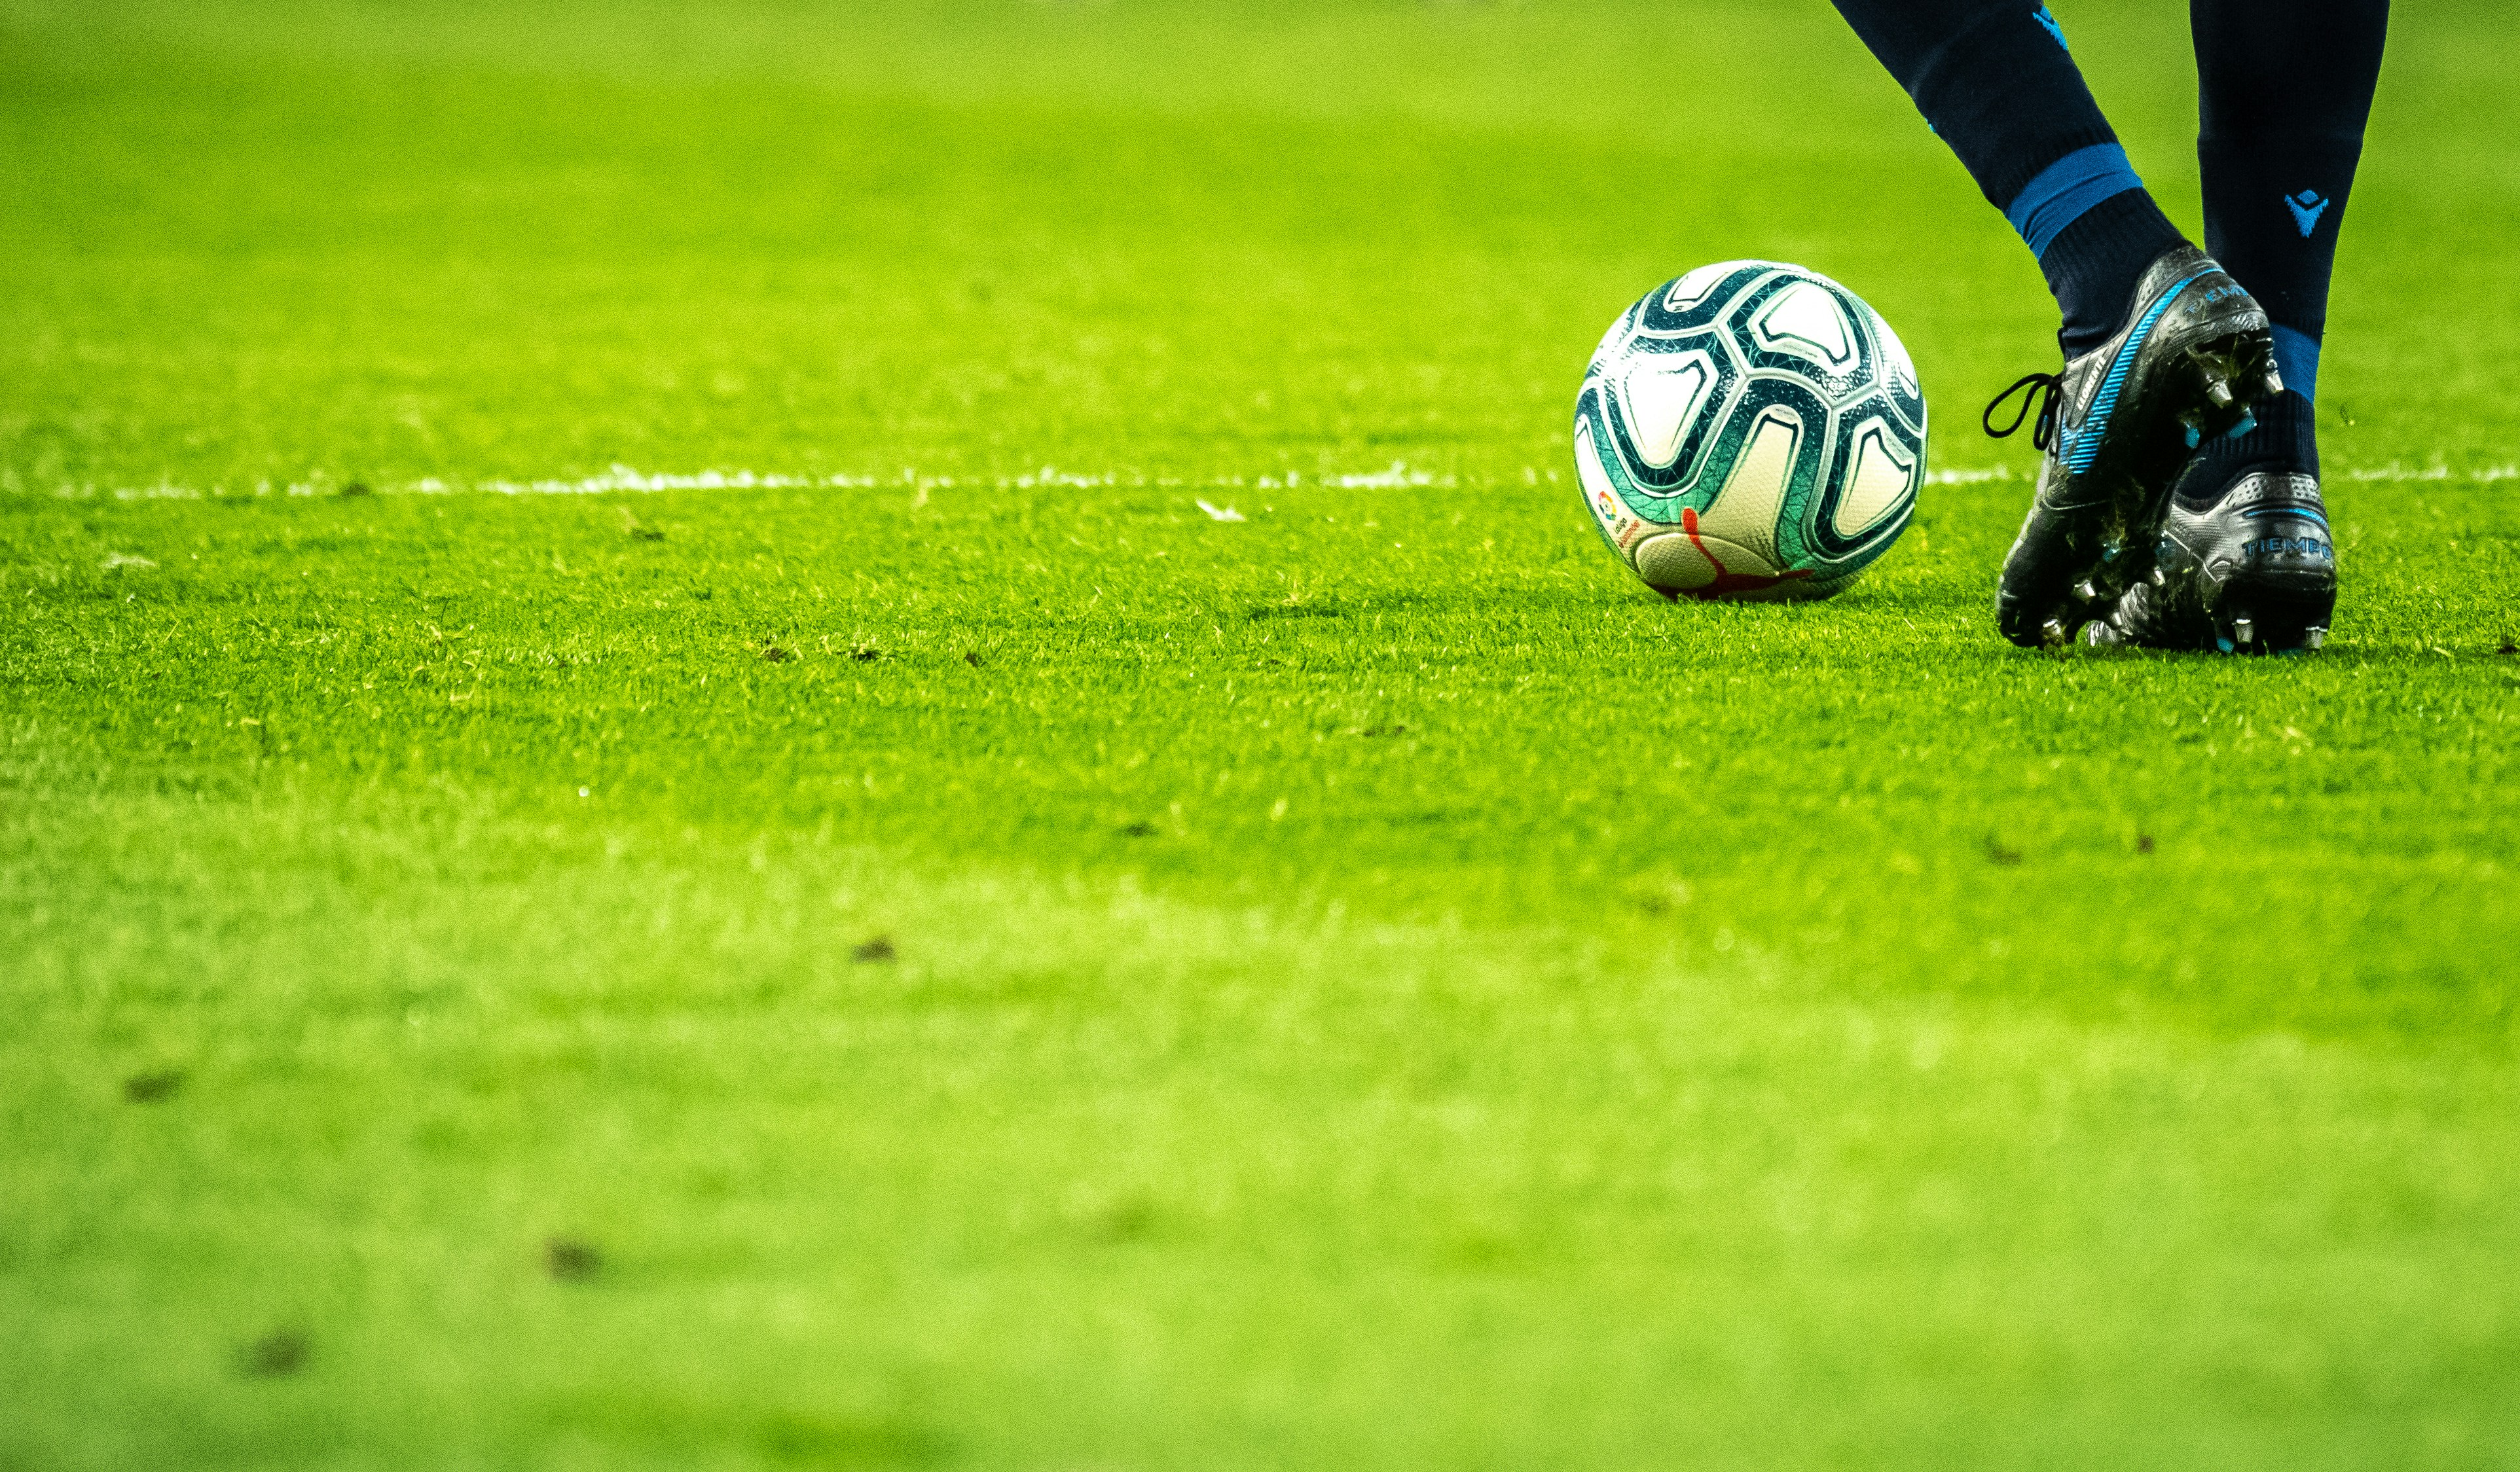
\includegraphics[width = 0.6\textwidth]{Billeder/fodbold}
	\end{center}
	Børge sparker til en fodbold. Sammenhængen mellem boldens højde over jorden $h$ og boldens vandrette afstand fra 
	Børge $x$ er givet ved
	\begin{align*}
		h(x) = -0.35x^2 + 1.067x, \  h > 0.
	\end{align*}
	Alle enheder er i meter. 
\end{opgavetekst}
\begin{delopgave}{1}
	Bestem boldens højde, når den har bevæget sig 10 meter væk fra Børge.
\end{delopgave}
\begin{delopgave}{2}
	Bestem boldens vandrette afstand fra Børge, når bolden lander på jorden igen. 
\end{delopgave}